% ============================================================
%  fmri-pipeline — Manuscript Draft
%  Compile: pdflatex paper && bibtex paper && pdflatex paper && pdflatex paper
% ============================================================
\documentclass[12pt]{article}

% --- packages ---
\usepackage[margin=1in]{geometry}
\usepackage{amsmath, amssymb}
\usepackage{graphicx}
\usepackage{booktabs}
\usepackage{array}
\usepackage{tabularx}
\usepackage{caption}
\usepackage{hyperref}
\usepackage[numbers, sort&compress]{natbib}
\usepackage{setspace}
\usepackage{parskip}
\usepackage{microtype}
\usepackage{xcolor}
\usepackage{enumitem}
\usepackage{rotating}   % sidewaysfigure for wide panels

% --- hyperref setup ---
\hypersetup{
  colorlinks = true,
  linkcolor  = blue!60!black,
  citecolor  = blue!60!black,
  urlcolor   = blue!60!black,
}

% --- section formatting (no titlesec required) ---
\makeatletter
\renewcommand\section{%
  \@startsection{section}{1}{\z@}%
    {14pt \@plus 4pt \@minus 2pt}%
    {1pt}%
    {\normalfont\large\bfseries\color{black}}}
\renewcommand\subsection{%
  \@startsection{subsection}{2}{\z@}%
    {10pt \@plus 2pt \@minus 1pt}%
    {4pt}%
    {\normalfont\normalsize\bfseries}}
\makeatother

% --- misc ---
\setstretch{1.15}
\captionsetup{font=small, labelfont=bf, width=0.92\textwidth}

% ============================================================
\begin{document}

% --- Title block ---
\begin{center}
  {\large\bfseries
    A Configuration-Driven Python Pipeline for Reproducible\\
    Functional Brain Network Analysis: Internal Validation\\
    on a Public fMRI Dataset}

  \vspace{10pt}
  {\normalsize Sara Pradhan}\\[2pt]
  {\small Mountain View High School, Mountain View, California}\\
  {\small \href{mailto:pradhan.sara@gmail.com}{pradhan.sara@gmail.com}}
\end{center}

\vspace{6pt}
\rule{\linewidth}{0.6pt}

% ============================================================
\section*{Abstract}
\noindent\rule{\linewidth}{0.4pt}\vspace{2pt}

\noindent\textbf{Background:}
Functional magnetic resonance imaging (fMRI) lets researchers estimate
coordinated activity across brain regions, but turning raw scanner data
into interpretable network metrics requires a chain of analysis
decisions (confound regression, parcellation, connectivity estimation,
and statistical testing), each of which can change the result. This
analytical flexibility is a particular obstacle for student
investigators, who often assemble custom scripts with little guidance on
which choices matter or how to document them.

\noindent\textbf{Question:}
Can a modular, YAML-configured Python pipeline recover established
features of large-scale brain organization and produce internally
reproducible outputs when applied to a publicly available fMRI dataset?

\noindent\textbf{Findings:}
I validated \texttt{fmri-pipeline} on a five-run subset of OpenNeuro
ds007318 (3~participants, working-memory task fMRI treated as
pseudo-resting-state). The pipeline recovered canonical network
organization, confirmed by a permutation test (within-network
$\bar{r} = 0.43$ vs.\ between-network $\bar{r} = 0.21$, gap $= 0.22$,
$p < 0.001$) and a corroborating edge-level analysis using the same
edges and network labels (Spearman $\rho = 0.32$, 95\% CI
$[0.31, 0.34]$). Regional homogeneity profiles were highly stable
within subjects across runs (within $\bar{r} = 0.97$ vs.\ between
$\bar{r} = 0.51$, from 2~within-subject run pairs). Static functional
connectivity showed a within-subject advantage (within $\bar{r} = 0.71$
vs.\ between $\bar{r} = 0.43$ across only 2~within-subject run pairs;
bootstrap 95\% CI on the gap $[0.22, 0.35]$). A parcellated
temporal-ICA proxy was stable across random seeds (20/20 components,
mean $|r| = 0.88$), though stability across leave-one-run-out subsets
was substantially weaker (mean $|r| = 0.411$, descriptive only given
$n \leq 3$ subsets). In a sensitivity analysis, global signal
regression (GSR) was the only tested parameter that substantially
altered connectivity estimates (Spearman $\rho = 0.862$ vs.\ baseline);
all other tested parameters produced near-identical outputs
($\rho \geq 0.99$). All statistics above reflect the GSR-on baseline
configuration.

\noindent\textbf{Significance:}
This is an engineering and reproducibility validation, not a
biological-discovery study. On a small public dataset,
\texttt{fmri-pipeline} produced internally consistent, biologically
plausible outputs with complete analytical transparency through a single
plain-text configuration file and an automatic validation scorecard,
lowering the barrier to reproducible fMRI analysis for student
investigators.

\rule{\linewidth}{0.4pt}

% ============================================================
\section{Introduction}

My interest in brain networks began with watching a family member live
with a serious mental illness, and with how hard it was for the
people around her to recognize what was happening until a crisis made it
impossible to miss. I did not set out to study her condition, and this
project does not: the dataset and sample size here cannot support
clinical claims of any kind, and I make none. What stayed with me was a
simpler question. When a brain-imaging analysis produces a number, how
do we know that number reflects the brain and not just the choices we
made along the way? That question is what led me to build and test a
transparent, reproducible analysis pipeline rather than simply run an
existing one.

Functional MRI allows researchers to estimate coordinated activity
across brain regions, but the path from BOLD images to interpretable
network results runs through many analysis choices. Reasonable teams can
make different decisions about confound regression, motion scrubbing,
spatial smoothing, atlas resolution, and statistical modeling, and the
``many analysts'' literature has shown that this flexibility can produce
substantially different conclusions even when teams start from the same
dataset~\citep{botvinik2020variability}. For a student researcher the
problem is sharper: a script can run cleanly while still producing
outputs that are undocumented, sensitive to arbitrary parameter choices,
or hard to reproduce. This raises a concrete, testable question: can a
pipeline built around transparent parameterization and built-in
internal-validity checks recover established features of large-scale
brain organization and produce outputs that are stable across runs and
analytical choices?

Several open-source tools already address parts of this workflow.
fMRIPrep standardizes functional
preprocessing~\citep{esteban2019fmriprep}, nilearn provides
connectivity estimation in Python~\citep{abraham2014machine}, and
BrainIAK offers advanced methods such as intersubject
correlation~\citep{kumar2021brainiak}. Integrated environments such as
the CONN toolbox~\citep{whitfield2012conn} and
XCP-D~\citep{mehta2024xcpd} provide broader end-to-end processing.
These tools are valuable, but they do not remove the need for a
project-specific layer that records every parameter choice, links the
analysis modules together, and checks whether outputs pass basic
internal-validity tests before biological interpretation, and none
provides a built-in scorecard designed for a student to confirm pipeline
validity before drawing conclusions.

I developed \texttt{fmri-pipeline} to fill that gap. All parameters
live in a single YAML file, analysis modules run in dependency order,
and a built-in reproducibility suite systematically tests whether
outputs meet expected internal-consistency criteria. By ``multi-scale''
I mean analyses spanning the local (voxelwise regional homogeneity) and
large-scale network (ROI-level functional connectivity) levels within
one workflow. The design goal is not to replace mature neuroimaging
packages but to make a complete, student-accessible workflow transparent
and self-checking. I tested three hypotheses: (1)~the pipeline recovers
canonical network organization, measured as stronger within-network than
between-network functional connectivity; (2)~local and network-level
outputs show higher within-subject than between-subject similarity
across repeated runs; and (3)~static FC estimates are mostly stable
across common parameter changes, except for known high-impact choices
such as global signal regression.

% ============================================================
\section{Materials and Methods}

\subsection{Dataset}

I used OpenNeuro dataset ds007318, a BIDS-formatted fMRI dataset for a
working-memory ``removal'' task with encoding, maintenance, removal,
and rest trial types, as defined in the dataset's
\texttt{task-removal\_events.json}
file~\citep{wang2026ds007318}.

The dataset's own documentation is internally inconsistent about sample
size: its README states ``Subjects: 43,'' while the OpenNeuro
landing-page metadata panel separately lists 42 participants. This
manuscript follows the README and \texttt{participants.tsv}, which are
the authoritative BIDS sources, and reports 43 as the repository size;
this is a discrepancy in the source repository, not an error introduced
by this analysis. This validation used the first three participants and
a fixed set of five runs selected for usable coverage during
preprocessing:

\begin{table}[h]
\centering
\small
\begin{tabular}{lrllr}
\toprule
\textbf{Participant} & \textbf{Age} & \textbf{Sex} &
  \textbf{Group label} & \textbf{Runs analyzed} \\
\midrule
sub-01 & 23 & Female & patient & ses-1, ses-2 \\
sub-02 & 28 & Male   & patient & ses-1 \\
sub-03 & 17 & Female & patient & ses-1, ses-2 \\
\bottomrule
\end{tabular}
\end{table}

The analyzed sample is therefore $N = 3$ participants and 5~BOLD runs
(only a single run from sub-02 was included). This is
adequate for a pipeline-validation exercise but not for
population-level inference. All three analyzed participants are labeled
as patients, so no diagnostic group comparison was performed. Because
the validation focuses on within-subject reproducibility and canonical
network structure (neither of which requires a control group), the
absence of a healthy comparison group does not affect the conclusions
reported here, but it does mean these results should not be assumed to
generalize to healthy or true resting-state data.

The pipeline used fMRIPrep derivatives~\citep{esteban2019fmriprep} as
inputs (MNI152NLin2009cAsym space, 2~mm isotropic voxels). The
functional data were acquired on a 3~T United Imaging (UIH) scanner
using a 2D EPI sequence (TR~$= 2.0$~s, TE~$= 30$~ms, flip
angle~$= 90^\circ$, 2~mm slice thickness, 75~slices, phase-encoding
$j-$), with values read directly from the BIDS JSON sidecars. The task
BOLD data were treated as pseudo-resting-state: no task-evoked
regressors were modeled, and all connectivity analyses (FC, ReHo, ICA
proxy) were applied as resting-state-style analyses. This is a
reasonable choice for engineering validation but is not equivalent to
analyzing true resting-state data. I treated this as a deliberate
trade-off: these task runs were the data with usable coverage available
to me, and the validation targets here---within- versus between-network
separation and within-subject stability---do not depend on the
rest-versus-task distinction, so I judged the substitution acceptable
for an engineering validation while flagging it as a limit on
generalization.

All data were obtained from the public OpenNeuro repository
(OpenNeuro ds007318, snapshot v1.0.0, downloaded February 2026;
\url{https://openneuro.org/datasets/ds007318/versions/1.0.0}),
distributed under a CC0 license. This work is a secondary analysis of a
publicly available, fully de-identified dataset and involved no new
data collection or contact with participants; secondary use of openly
licensed, de-identified data of this kind does not constitute
human-subjects research requiring new ethical approval.

\subsection{Pipeline Overview}

\texttt{fmri-pipeline} accepts fMRIPrep derivatives in BIDS format and
is controlled entirely by a single YAML configuration file. The modules
exercised in this validation were: (1)~preprocessing quality-control
checks and confound regression; (2)~regional homogeneity (ReHo),
computed voxelwise as Kendall's coefficient of concordance over each
voxel's 26-neighbor cluster and summarized to ROI level using the atlas
parcellation~\citep{zang2004regional}; (3)~static functional
connectivity (FC), estimated as pairwise Pearson correlations followed
by Fisher-$z$ transformation across the Schaefer-200 atlas (200~ROIs,
7-network assignment, 2018 release, applied in MNI152NLin2009cAsym
space)~\citep{schaefer2018local, yeo2011organization}; (4)~exploratory
dynamic FC using a sliding-window approach across multiple window
lengths~\citep{damaraju2014dynamic}; (5)~a parcellated temporal-ICA
stability check~\citep{hyvarinen1999fast, kuhn1955hungarian};
(6)~graph-metric summaries of thresholded FC
matrices~\citep{bullmore2009complex}; and (7)~a sensitivity-analysis
module that systematically varies parameters and computes pairwise
Spearman correlations between the resulting connectivity vectors. The
pipeline additionally implements intersubject
correlation~\citep{kumar2021brainiak} and group-level mass-univariate
OLS with Benjamini--Hochberg FDR correction~\citep{benjamini1995controlling};
these modules were not exercised in this single-dataset, single-group
validation and are therefore not reported in the Results.

\subsection{Confound Regression and Quality Control}

Following fMRIPrep preprocessing, confound regression used six
rigid-body motion parameters (three translations, three rotations) and
their temporal derivatives (12~motion regressors), mean white-matter
signal, and mean CSF signal. Volumes with framewise displacement (FD)
exceeding 0.5~mm were flagged and excluded from downstream statistical
operations via NaN masking. Cleaned BOLD timeseries were
bandpass-filtered at $0.01$--$0.10$~Hz with a zero-phase Butterworth
filter and spatially smoothed with a 6~mm FWHM Gaussian kernel before
connectivity estimation (baseline condition). For the global signal
regression (GSR) sensitivity condition, a whole-brain mean BOLD
regressor was additionally appended to the confound matrix. GSR was
treated as a high-impact parameter because prior work shows it can
substantially change FC estimates and network
topology~\citep{power2012spurious, murphy2017towards}.

\textbf{Baseline note:} all within- versus between-network and
reproducibility statistics reported in the Results
(Table~\ref{tab:scorecard}) were computed under this GSR-on baseline
configuration. Because the sensitivity analysis below shows GSR is the
single parameter that substantially alters connectivity estimates
($\rho = 0.862$ relative to GSR-off), the specific gap magnitudes
reported here should not be assumed to hold under GSR-off
preprocessing; GSR status should be matched whenever these results are
compared against other pipelines or datasets.

\subsection{Functional Connectivity and the Network Anchor}

For each run the pipeline extracted Schaefer-200 ROI timeseries and
computed a $200 \times 200$ FC matrix; the upper triangle contained
19,900 unique ROI-pair values before masking invalid edges. One ROI in
sub-03 ses-2 had a zero-variance timeseries from incomplete brain
coverage and was excluded via NaN masking; all statistics used only
jointly valid edges. To test canonical organization, edges were divided
into within-network (both ROIs in the same Yeo/Schaefer network) and
between-network pairs, and mean within- vs.\ between-network FC was
compared with a permutation test (1,000 shuffles of the network-label
vector, two-tailed; $p$ lower-bounded at $1/1{,}000$). As a
complementary, effect-size-oriented view of the same
contrast---not an independent check, since it uses the identical edges
and network labels---I also computed the Spearman correlation between
Fisher-$z$ edge values and a same-network membership indicator
(3,093~within-network and 16,807~between-network edges).

\subsection{Reproducibility Analyses}

\textbf{FC reproducibility.}
For each subject I computed the upper-triangle FC vector per run, then
within-subject run-pair correlations and between-subject cross-run
correlations (Pearson $r$ on valid edges, pairwise NaN masking). I
compared within- to between-subject similarity with a one-sided Wilcoxon
rank-sum test and a bootstrap 95\% CI ($B = 1{,}000$ run-level
resamples) on the within-minus-between gap. Because only sub-01 and
sub-03 contributed repeated runs, this run-pair comparison was restricted
to those two subjects, yielding 2~within-subject and 4~between-subject run
pairs (sub-02's single run cannot form a within-subject pair and is
therefore excluded from this test, though it does enter the three-subject
ReHo comparison below). With only 2~within-subject and 4~between-subject
pairs, this test has theoretical power below 17\% even for large true
effects, so the bootstrap CI is treated as suggestive, not confirmatory,
evidence throughout this manuscript.

\textbf{ReHo stability.}
Per run, the ReHo map was computed from cleaned BOLD and summarized to
ROI level using the Schaefer-200 atlas; I compared within- to
between-subject run-to-run Pearson $r$ using the same bootstrap
procedure (2~within-subject pairs: sub-01 ses-1$\times$ses-2 and sub-03
ses-1$\times$ses-2; 8~between-subject pairs across all three subjects).
An early pipeline run wrote empty NIfTI stubs rather than valid ReHo
maps because of a bug in the output-writing module (corrected before
the archived release, v1.0.1); I recomputed ReHo from cleaned BOLD
using a brain mask derived from temporal variance, which is
methodologically equivalent to a gray-matter mask for ROI-level
extraction.

\textbf{ICA stability.}
I ran temporal FastICA~\citep{hyvarinen1999fast} on the group-averaged
Schaefer-200 ROI timeseries using 5~random seeds ($k = 20$) and matched
components across seeds with the Hungarian
algorithm~\citep{kuhn1955hungarian} on the absolute-correlation matrix;
a component was robust if $|r| \geq 0.70$ against all counterparts.
\textbf{This is a parcellated temporal-ICA proxy and does not directly
validate the pipeline's spatial-ICA module.} A leave-one-run-out
cross-validation yielded only 3~run subsets and is reported
descriptively only.

\textbf{Graph metric stability.}
From the group-average FC matrix I computed modularity (Louvain), global
efficiency, and clustering coefficient at density thresholds 0.10, 0.15,
and 0.20, with bootstrap resampling ($B = 500$) for 95\% CIs and the
coefficient of variation.

\textbf{Dynamic FC sensitivity.}
I computed sliding-window FC variability (SD of the upper-triangle
vector over time) at window lengths 20, 30, and 40~TRs, used
$k$-means ($k = 4$, $k$-means$++$, 10~restarts) to assign states within
each condition, and computed the Adjusted Rand Index (ARI) between
conditions.

\subsection{Sensitivity Analysis}

I tested output stability across 11~conditions spanning 5~dimensions:
GSR (on/off), atlas resolution (Schaefer-100/200/400), dynamic-FC
window length (20/30/45/60~TRs; this sweep uses a wider window grid than
the 20/30/40-TR reproducibility analysis above), motion scrubbing threshold
(FD~$= 0.3/0.5/0.9$~mm), and smoothing kernel (4/6/8~mm FWHM).
Baseline was Schaefer-200, GSR on, FD~0.5~mm, 6~mm smoothing,
30-TR window. For each condition I compared the static FC
upper-triangle vector to baseline with Spearman correlation. Note that
static FC does not depend on the dynamic-FC window length, so the
window-length conditions are identical to baseline ($\rho = 1.00$) by
construction and are reported only for completeness; the
atlas-resolution conditions produce FC vectors of a different length
(Schaefer-100/400 have different ROI counts than the Schaefer-200
baseline) and are therefore not directly edge-comparable to
baseline---no Spearman $\rho$ was computed for these conditions, and
Figure~\ref{fig:sensitivity} marks them ``N/T'' (not tested) rather
than showing a numeric value. The smoothing conditions apply the kernel
to the cleaned BOLD before ROI extraction. The
figure reports the 9~conditions with atlas resolution held constant
(so edges are directly comparable); all 11 are discussed in the
text, with the per-condition similarity table
(\texttt{recommended\_defaults.csv}) and the full pairwise similarity
matrix (\texttt{stability\_matrix\_static\_fc.npy} with
\texttt{stability\_labels.csv}) provided in the archived repository.

\subsection{Software and Statistics}

\texttt{fmri-pipeline} is implemented in Python ($\geq$~3.8) and
depends on \texttt{numpy}, \texttt{scipy}, \texttt{pandas},
\texttt{nilearn}, \texttt{nibabel}, \texttt{statsmodels},
\texttt{scikit-learn}, and \texttt{pyyaml}. Group-level testing uses
mass-univariate OLS with Benjamini--Hochberg FDR
correction~\citep{benjamini1995controlling}. All stochastic operations
used deterministic seeds set in the configuration file. The test suite
validates core computations on synthetic data and requires no
neuroimaging files to run.

% ============================================================
\section{Results}

\subsection{Data Quality}

All five runs passed the predefined motion-quality criteria
(mean FD~$< 0.5$~mm, percent scrubbed~$< 20\%$). Mean FD ranged from
0.101 to 0.150~mm, and only sub-02 ses-1 had any scrubbed volumes
($\approx\!1.2\%$) at the FD~$> 0.5$~mm threshold (Table~\ref{tab:qc}).
DVARS ranged from 3.68 to 4.41 across runs. One ROI in sub-03 ses-2
had a zero-variance timeseries and was excluded via NaN masking.

\begin{table}[h]
\centering
\small
\caption{Run-level motion quality-control summary at the FD~0.5~mm
  scrubbing threshold. All runs passed pipeline exclusion criteria.}
\label{tab:qc}
\begin{tabular}{lrrrr}
\toprule
\textbf{Run} & \textbf{Mean FD (mm)} & \textbf{Median FD (mm)} &
  \textbf{Scrubbed (\%)} & \textbf{DVARS} \\
\midrule
sub-01, ses-1 & 0.105 & 0.096 & 0.00 & 3.73 \\
sub-01, ses-2 & 0.101 & 0.095 & 0.00 & 3.68 \\
sub-02, ses-1 & 0.144 & 0.119 & 1.18 & 4.41 \\
sub-03, ses-1 & 0.122 & 0.103 & 0.00 & 3.85 \\
sub-03, ses-2 & 0.150 & 0.121 & 0.00 & 3.95 \\
\bottomrule
\end{tabular}
\end{table}

\subsection{Canonical Network Organization Is Recovered}

The strongest validation result was the recovery of canonical
large-scale network organization. Mean within-network FC
($\bar{r} = 0.43$) substantially exceeded mean between-network FC
($\bar{r} = 0.21$) across all seven canonical Yeo networks, a gap of
0.22 ($p < 0.001$, permutation test, 1,000~shuffles; $p$ at the
minimum resolvable value of $1/1{,}000$).

\textbf{Spatial autocorrelation caveat:} the Schaefer-200 parcellation
assigns ROIs by functional similarity, but Yeo-network labels remain
spatially contiguous to a meaningful degree, and the label-shuffling
permutation test used here does not preserve or destroy spatial
structure. It therefore cannot, by itself, rule out a contribution from
spatial autocorrelation (e.g., smoothing-induced proximity correlations)
to the observed within-network effect. A spatially-constrained
(``spin test'') permutation, which preserves the geometry of the
cortical surface while shuffling network identity, would be needed to
more rigorously isolate the network-driven component of this effect;
that test was not run for this validation and is flagged as a priority
follow-up rather than a settled conclusion.

As an effect-size restatement of the same within- versus
between-network contrast---using the identical edges and network
labels, not an independent check---the Spearman correlation between
Fisher-$z$ edge values and same-network membership was $\rho = 0.32$
(95\% CI $[0.31, 0.34]$), confirming that same-network ROI pairs are
systematically more connected than cross-network pairs across the full
edge distribution.

Within-network FC was highest for the Visual (Fisher-$z$, $M = 0.72$)
and Dorsal Attention ($M = 0.49$) networks, consistent with strong
local synchrony commonly reported in unimodal sensory and attention
systems, followed by Somatomotor ($M = 0.45$), Salience/Ventral
Attention ($M = 0.39$), Default Mode ($M = 0.35$), and Frontoparietal
($M = 0.33$); the Limbic network was weakest ($M = 0.17$), consistent
with the lower BOLD signal-to-noise ratio typically reported in limbic
regions. No specific canonical rank ordering was pre-registered for
this comparison, so this ordering is reported descriptively rather than
as a validated match to an external benchmark. Because the data are
task fMRI treated as pseudo-resting-state, this is best read as
evidence of biologically plausible network structure rather than proof
that task-state FC matches resting-state architecture
(Figure~\ref{fig:fc_matrix}).

\begin{figure}[p]
  \centering
  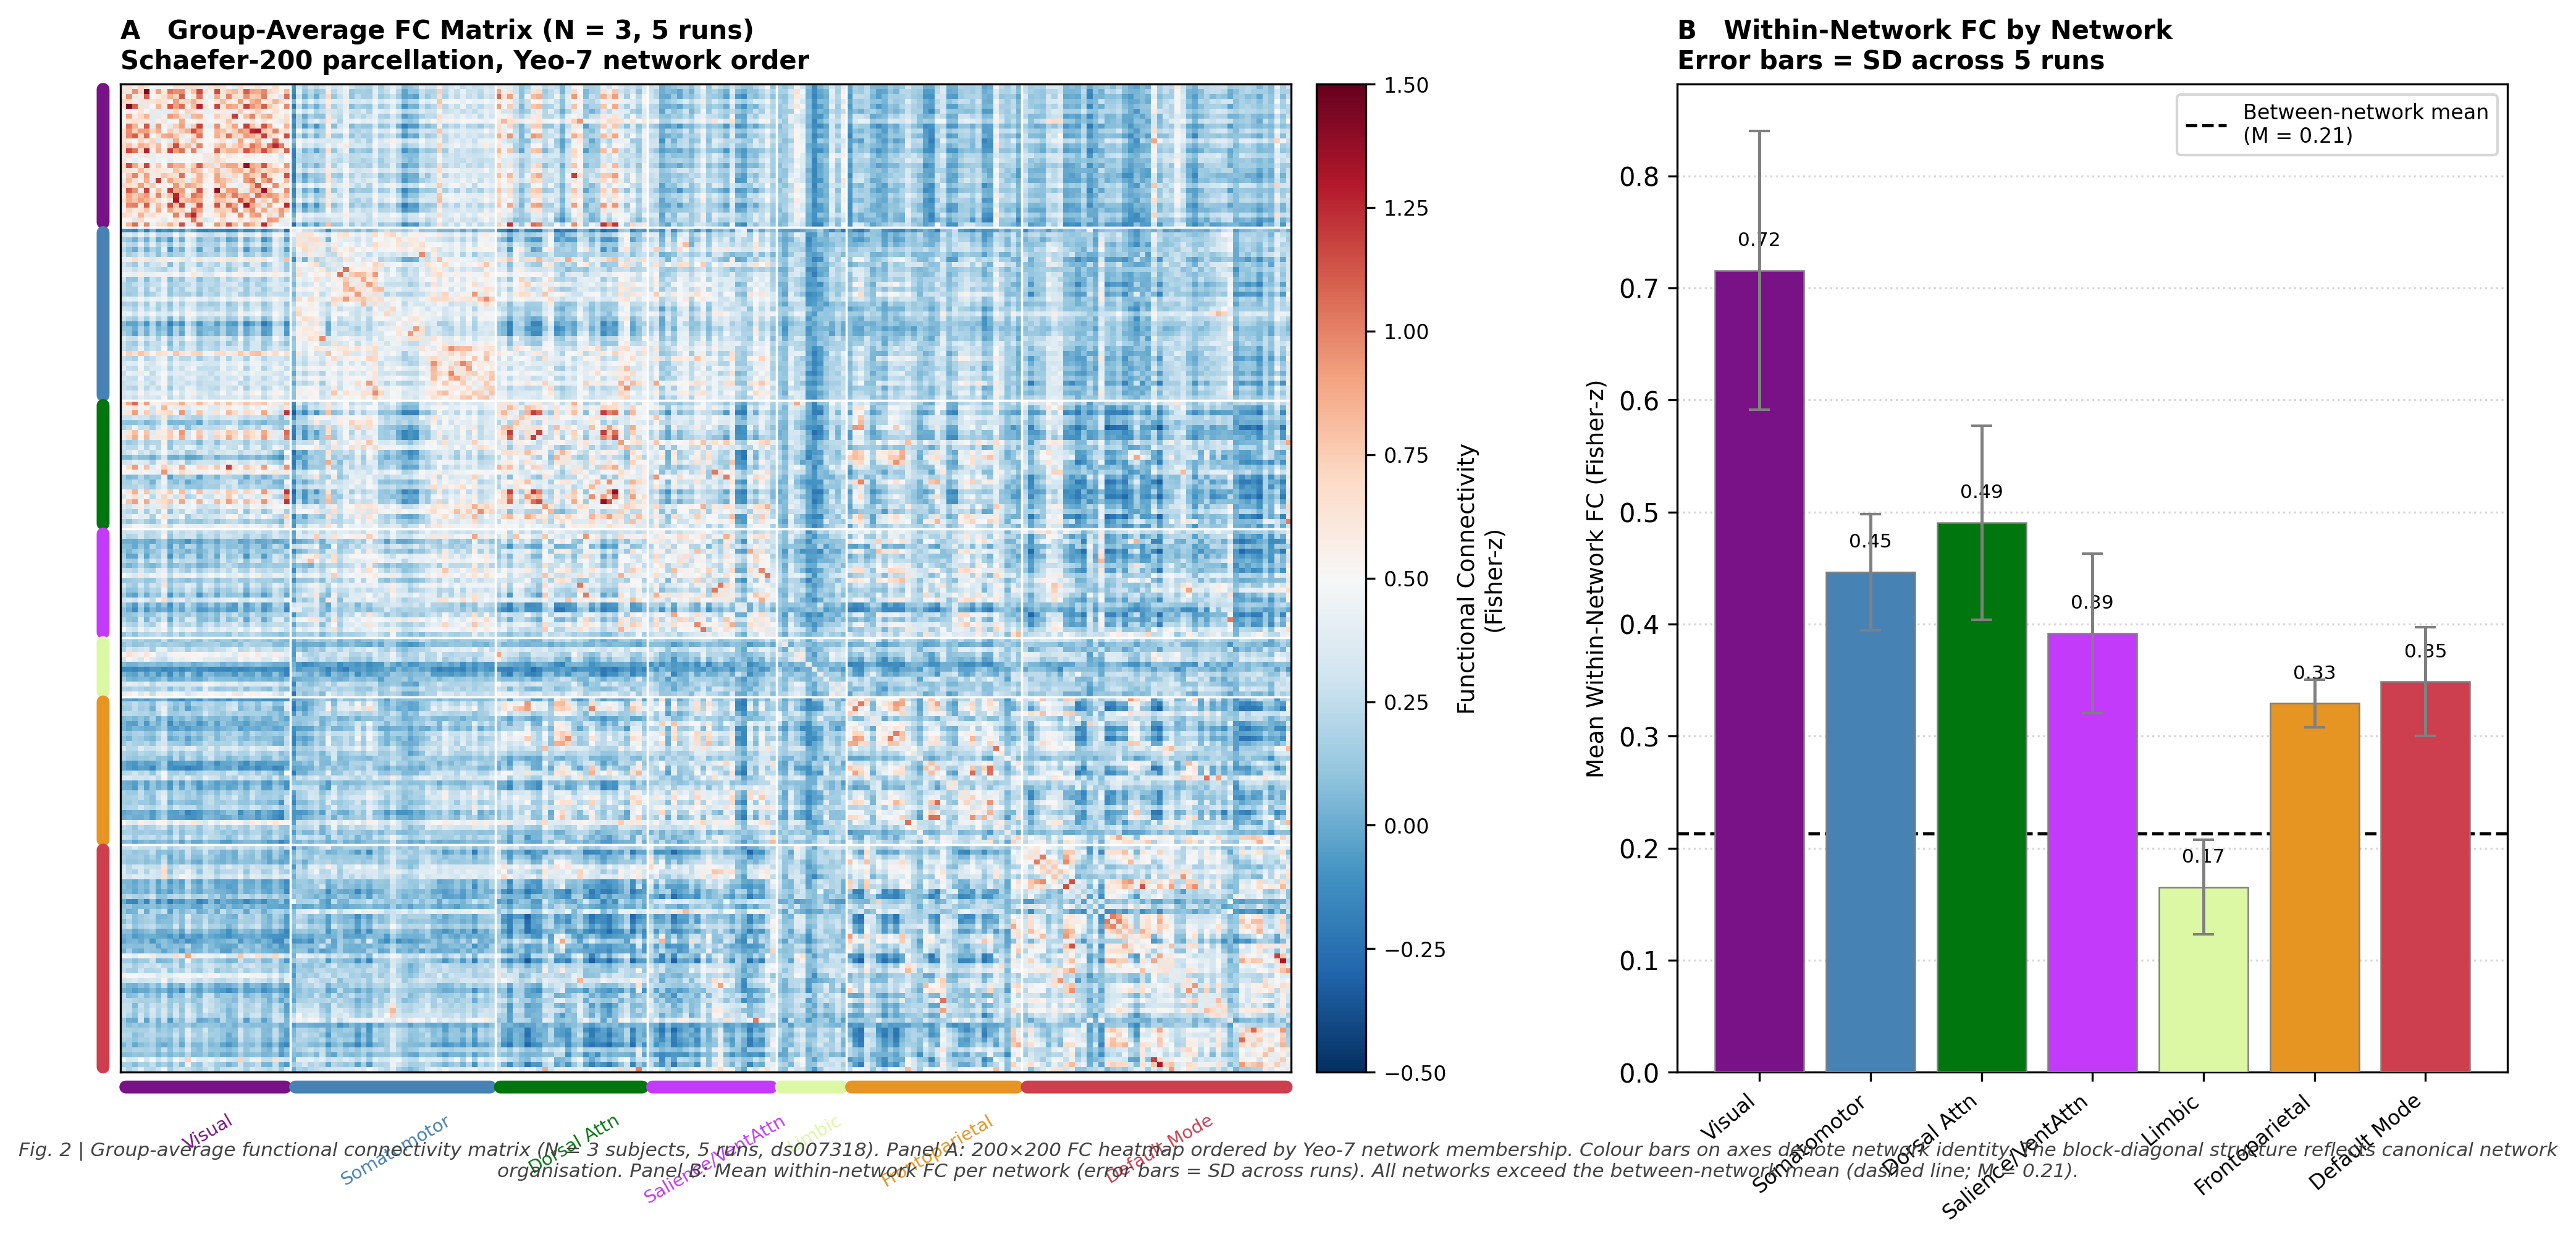
\includegraphics[width=\textwidth]{figures/fc_matrix_canonical.png}
  \caption{Group-average functional connectivity matrix ($N = 3$
    subjects, 5~runs, ds007318). \textbf{Panel~A:} $200 \times 200$
    FC heatmap ordered by Yeo-7 network membership (Schaefer-200
    parcellation, Fisher-$z$ scale, clipped to $[-0.5,\, 1.5]$);
    axis colour bars denote network identity. The block-diagonal
    structure reflects canonical large-scale network organization.
    \textbf{Panel~B:} Mean within-network FC per canonical network;
    error bars show SD across the 5~runs. All networks exceed the
    between-network mean (dashed line; $M = 0.21$).
    Vis~$=$~Visual; SomMot~$=$~Somatomotor;
    DorsAttn~$=$~Dorsal Attention;
    SalVentAttn~$=$~Salience/Ventral Attention;
    Cont~$=$~Frontoparietal/Control; Limbic~$=$~Limbic;
    DMN~$=$~Default Mode.}
  \label{fig:fc_matrix}
\end{figure}

\begin{figure}[p]
  \centering
  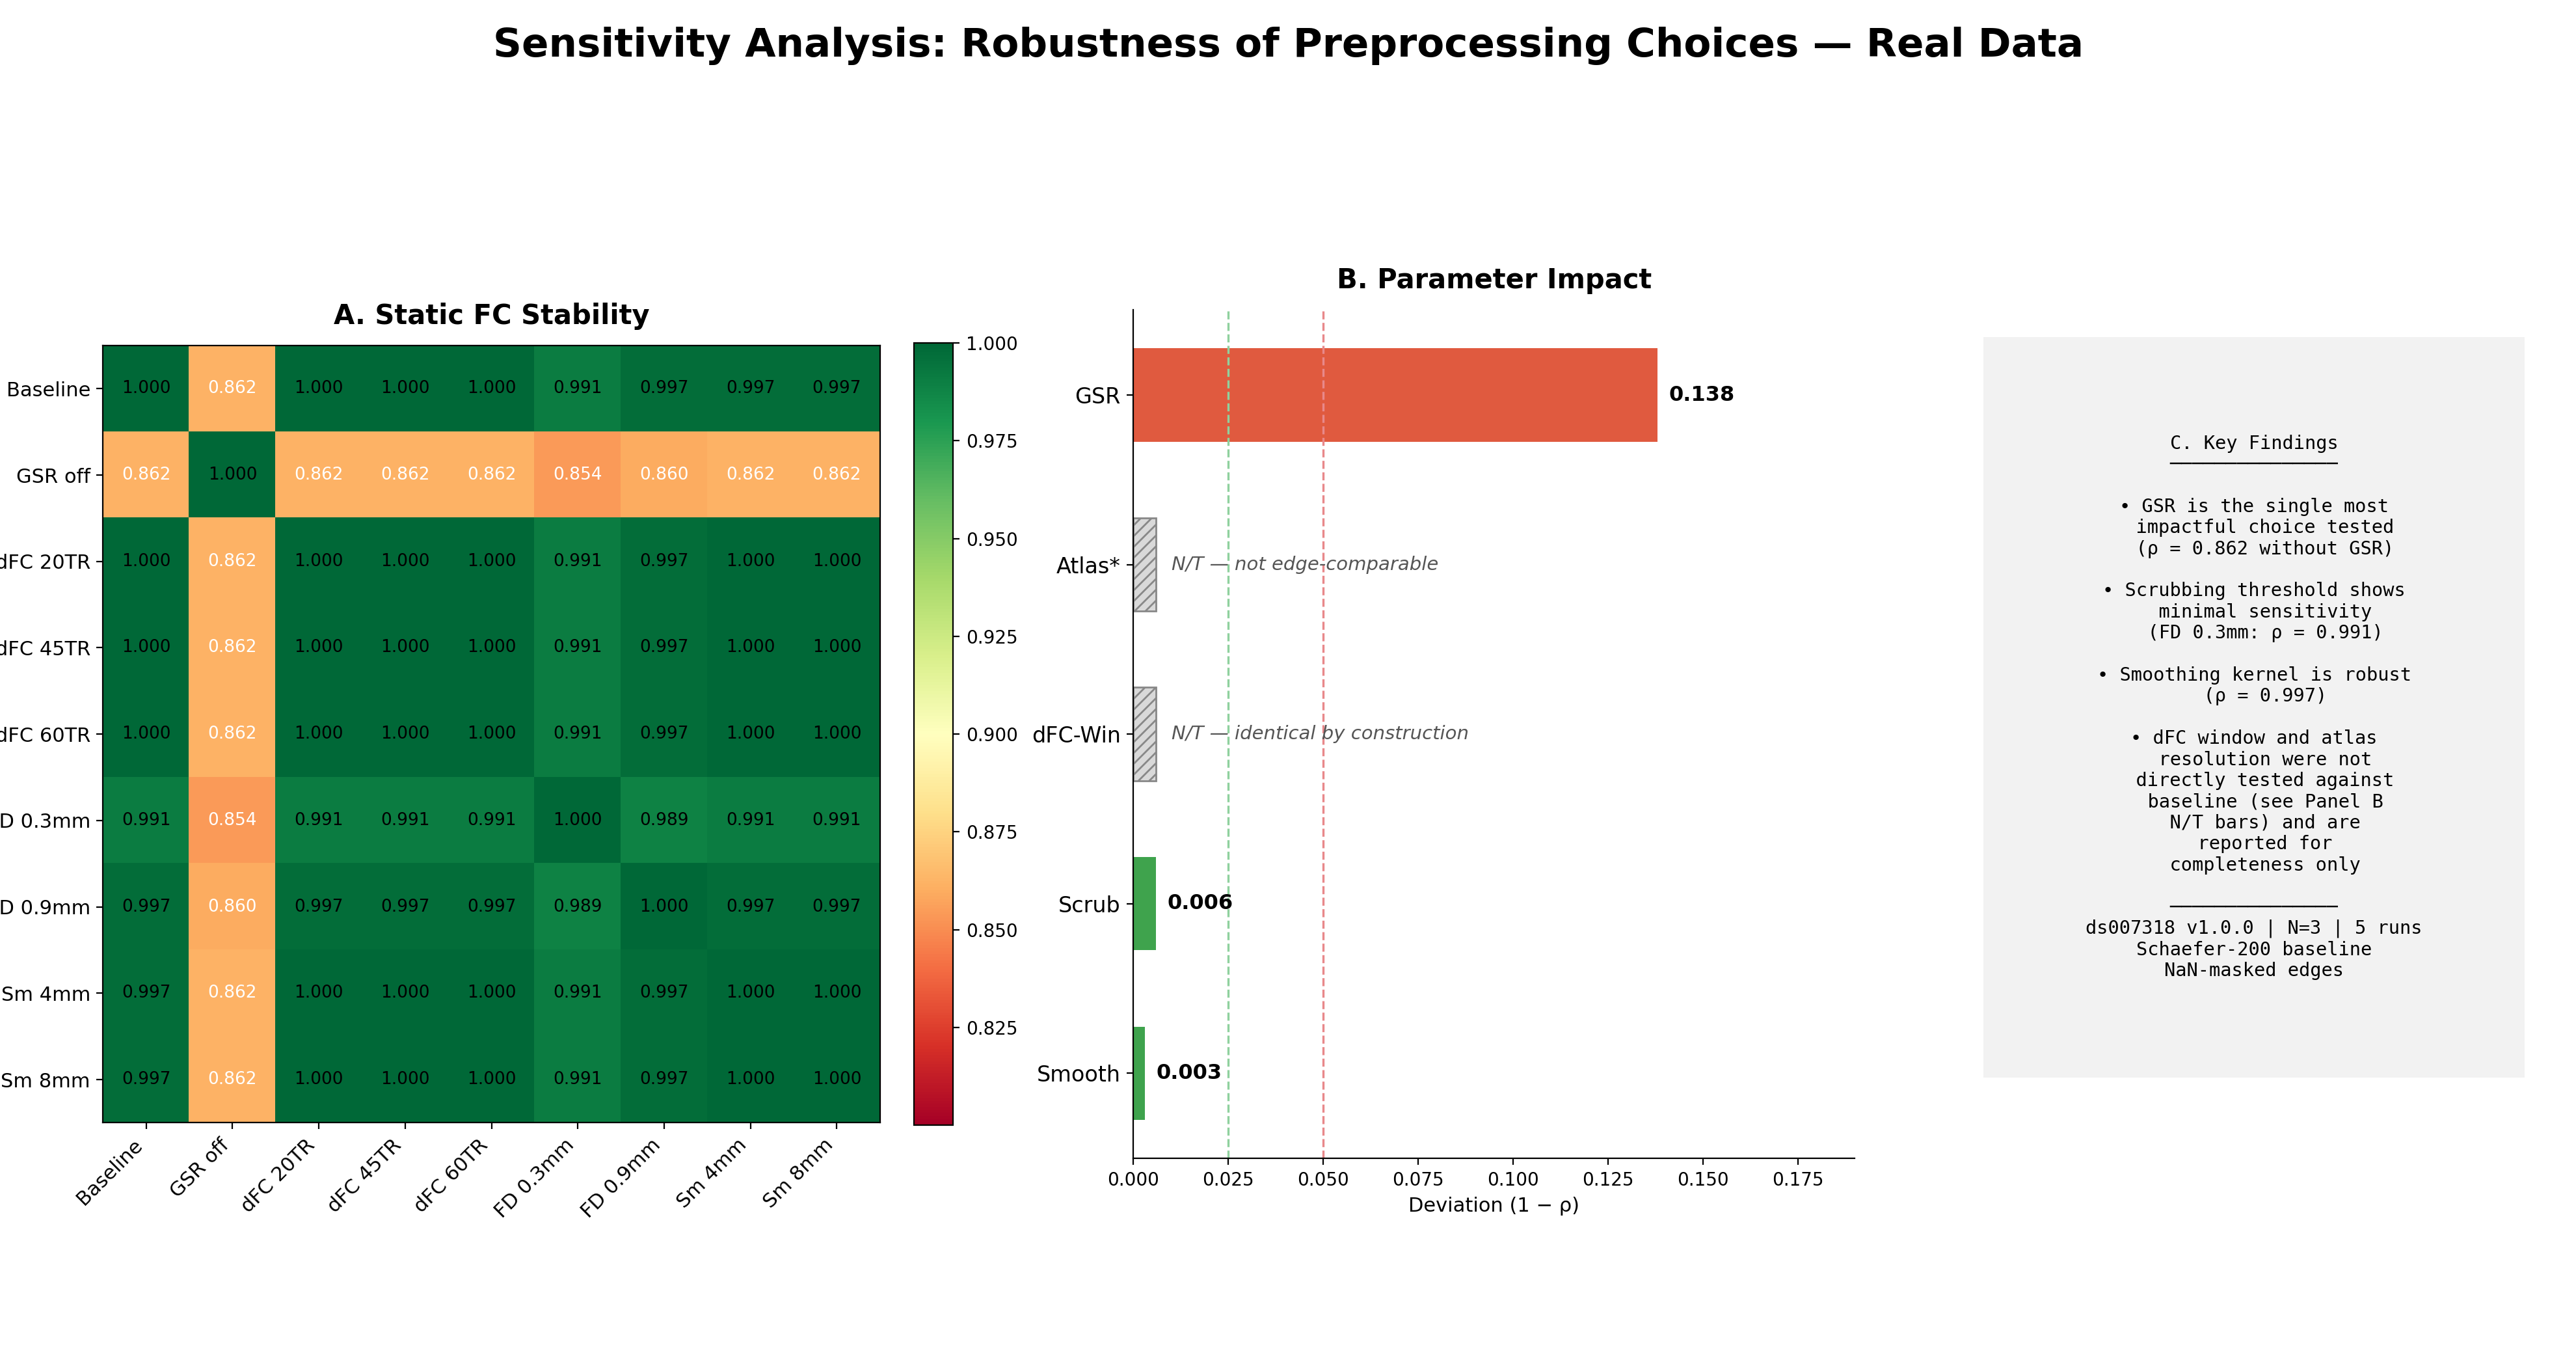
\includegraphics[width=\textwidth]{sensitivity_figures_real/joss_figure_sensitivity_combined.png}
  \caption{Sensitivity analysis from ds007318 ($N = 3$, 5~runs).
    \textbf{A.}~Pairwise Spearman correlation matrix for static FC
    vectors across 9~parameter conditions (Schaefer-200, varying GSR,
    scrubbing threshold, window length, smoothing kernel); all
    conditions except GSR-off produce $\rho > 0.99$ (window-length
    conditions are identical to baseline by construction, as static FC
    does not depend on the dynamic-FC window).
    \textbf{B.}~Parameter impact as mean deviation from baseline
    ($1 - \rho$) for the three parameters actually tested against
    baseline on comparable edges (GSR, scrubbing threshold, smoothing
    kernel). The dFC-window and atlas-resolution conditions are not
    shown as numeric bars: dFC-window is identical to baseline by
    mathematical construction (not a real robustness test), and
    atlas-resolution conditions produce FC vectors of a different
    length that cannot be correlated edge-for-edge against the
    Schaefer-200 baseline. Both are marked ``N/T'' (not tested) rather
    than assigned a misleading 0.000 value.
    \textbf{C.}~Summary of key findings, updated to match Panel~B.}
  \label{fig:sensitivity}
\end{figure}

\subsection{Internal Reproducibility Analyses}

Table~\ref{tab:scorecard} summarizes the reproducibility analyses,
described below in order of evidential strength.

\begin{table}[htbp]
\centering
\small
\caption{Validation scorecard for \texttt{fmri-pipeline} on OpenNeuro
  ds007318 ($N = 3$ subjects, 5~runs). Seed stability and cross-run
  stability of the temporal-ICA proxy are reported as separate rows so
  a strong seed result cannot mask a weaker cross-run result. Rows
  marked ``suggestive'' rest on bootstrap CIs built from only
  2~within-subject pairs and should not be read as precise interval
  estimates. CI~$=$~bootstrap 95\% confidence interval ($B = 1{,}000$
  run-level resamples). n/a~$=$~not assessable at this sample size.}
\label{tab:scorecard}
\begin{tabular}{p{2.7cm} p{3.1cm} p{3.0cm} p{1.9cm} p{2.2cm}}
\toprule
\textbf{Dimension} & \textbf{Metric} & \textbf{Result} &
  \textbf{CI (gap)} & \textbf{Status} \\
\midrule
Static FC plausibility &
  Canonical network organization &
  within $\bar{r}=0.43$, between $\bar{r}=0.21$, gap~$=0.22$,
  $p<0.001$ &
  --- & \checkmark \\[4pt]

ReHo stability &
  Cross-run spatial similarity (2 within / 8 between pairs) &
  within $\bar{r}=0.97$, between $\bar{r}=0.51$ &
  $[0.436, 0.480]$ & \checkmark\ (suggestive, $n=2$) \\[4pt]

ICA seed stability (temporal proxy) &
  Component recovery across seeds &
  20/20 robust, mean $|r|=0.88$ &
  --- & \checkmark\ (seed only) \\[4pt]

ICA cross-run stability (LORO-CV) &
  Component recovery across run subsets &
  mean $|r|=0.411$ (3 subsets) &
  --- & \textbf{$\times$}\ Fails $|r|\!\geq\!0.70$ \\[4pt]

FC reproducibility &
  Within- vs.\ between-subject (2 within / 4 between pairs) &
  within $\bar{r}=0.71$, between $\bar{r}=0.43$, $p=0.067$ &
  $[0.217, 0.348]$ & \checkmark\ (suggestive, $n=2$) \\[4pt]

Graph metric stability &
  Bootstrap CI on modularity &
  $Q=0.447$, 95\% CI $[0.391, 0.503]$, CV~$=17\%$ &
  --- & \checkmark \\[4pt]

Dynamic FC robustness &
  Multi-window ARI &
  ARI $0.42$--$0.57$ &
  --- & n/a (exploratory) \\
\bottomrule
\end{tabular}
\end{table}

\textbf{ReHo stability} was the strongest reproducibility result.
Within-subject run-to-run Pearson $r$ for ROI ReHo profiles was
$0.97$ versus $0.51$ between subjects (2~within-subject pairs vs.\
8~between-subject pairs; gap~$= 0.455$, 95\% CI $[0.436, 0.480]$). The
near-perfect within-subject similarity indicates the ReHo spatial
pattern is highly consistent across runs, and the large gap shows
individual differences are preserved. Standardizing this gap yields a
numerically enormous Cohen's $d$ ($\approx 31$), but at $N = 3$ that
value is an artifact of near-ceiling within-subject similarity rather
than a meaningful reliability estimate, so I report the raw within- and
between-subject means, the pair counts, and the bootstrap CI as the
interpretable quantities---read as suggestive given the very small
number of within-subject pairs, not as a precise population estimate.

\textbf{ICA stability} across random seeds was strong: all 20
components were robustly recovered ($|r| \geq 0.70$) across all
5~seeds, mean $|r| = 0.88$, indicating the temporal decomposition is
not sensitive to initialization. This validates seed stability of the
parcellated temporal-ICA proxy only, not the spatial-ICA module. The
LORO-CV (3~run subsets) told a different story: mean $|r| = 0.411$,
well below the $0.70$ robustness threshold used for seed stability,
consistent with the known instability of temporal ICA on very small
datasets. Because these two tests probe different kinds of robustness,
Table~\ref{tab:scorecard} reports them as separate scorecard
rows---seed stability passes, cross-run (LORO-CV) stability does
not---so the strong seed result does not mask the weaker cross-run
result.

\textbf{FC reproducibility} showed a consistent within-subject
advantage: within-subject run-pair FC correlation $\bar{r} = 0.71$
($n = 2$~pairs) versus between-subject $\bar{r} = 0.43$ ($n = 4$~pairs),
a gap of 0.28. The bootstrap 95\% CI on the gap $[0.217, 0.348]$
excludes zero. The Wilcoxon rank-sum test did not reach significance
($p = 0.067$), but with only 2~within-subject pairs it is severely
underpowered. Given that the bootstrap CI itself rests on only
2~within-subject pairs, it is offered here as supporting, not
definitive, evidence of a within-subject advantage.

\textbf{Graph metric stability} was adequate. Bootstrap resampling
($B = 500$) of modularity at density 0.15 gave $Q = 0.447$
(95\% CI $[0.391, 0.503]$, CV~$= 17\%$). No published consensus CV
threshold exists for this context; 17\% is reported descriptively. The
observed $Q$ falls within the range commonly reported for resting-state
networks at comparable atlas resolutions~\citep{bullmore2009complex},
providing an external anchor for the observed network separation.

\subsection{Sensitivity to Preprocessing Parameters}

Global signal regression was the only parameter that substantially
altered connectivity estimates (Spearman $\rho = 0.862$ relative to
baseline), consistent with the established literature on GSR's effect
on FC topology~\citep{power2012spurious, murphy2017towards}. Of the
parameters actually tested against a comparable baseline, all others
produced near-identical static FC outputs when atlas resolution was
held constant: smoothing-kernel variations were very close to baseline
(4~mm: $\rho = 0.997$; 8~mm: $\rho = 0.997$), and scrubbing-threshold
variations remained very high (FD~$= 0.3$~mm: $\rho = 0.991$;
FD~$= 0.9$~mm: $\rho = 0.997$). Window-length variations are identical
to baseline by construction ($\rho = 1.00$, since static FC does not
depend on the dynamic-FC window) and atlas-resolution conditions were
not edge-comparable to baseline, so neither is treated as a genuine
robustness test (see Figure~\ref{fig:sensitivity} caption). With the
exception of GSR, the pipeline's static FC outputs were robust
($\rho \geq 0.99$) across the preprocessing parameters that could be
directly tested against baseline in this low-motion subset
(Figure~\ref{fig:sensitivity}).

Dynamic FC variability (upper-triangle SD over time) decreased
monotonically with window size ($W = 20$~TR: $0.409$;
$30$~TR: $0.308$; $40$~TR: $0.253$), as expected from the averaging
properties of longer windows. State-assignment consistency across window
lengths was moderate (ARI $0.42$--$0.57$), reflecting the dependence of
sliding-window clustering on temporal resolution. Dynamic FC outputs are
included for exploratory characterization only and are not the basis for
state-based inference at this sample size.


% ============================================================
\section{Discussion}

\subsection{Principal Findings}

\texttt{fmri-pipeline} produced coherent, internally reproducible
functional-network outputs from a small public fMRI dataset without
modification of source code; only the YAML configuration was changed
to point at the new data. The strongest result---recovery of canonical
network organization confirmed by a permutation test ($p < 0.001$) and
corroborated by an effect-size restatement of the same contrast
($\rho = 0.32$)---establishes that the pipeline's FC matrices are
biologically plausible: within-network connections are systematically
stronger than between-network connections across all seven Yeo
networks, though spatial autocorrelation has not been formally ruled
out as a partial contributor (see Results). This is the expected
signature of large-scale brain
modularity~\citep{bullmore2009complex}, and its recovery is consistent
with correct functioning of the atlas-parcellation and
connectivity-estimation steps.

The reproducibility analyses collectively indicate the outputs are not
arbitrary, though the within-subject sample size (2~repeated-run pairs)
limits how strongly this can be stated. ReHo profiles were nearly
perfectly reproduced within subjects across runs; static FC showed a
within-subject advantage with a bootstrap CI that excludes zero,
treated here as suggestive rather than confirmatory; and the
parcellated temporal-ICA proxy was stable across seeds but not across
leave-one-run-out subsets. The paper's strongest defensible claim is that
the pipeline produced biologically plausible and internally reproducible
outputs on a small public subset, supporting its use as a transparent
validation workflow for future, larger analyses. The current data do
\textbf{not} support claims of disease-biomarker discovery,
schizophrenia-related dysconnectivity, or general test-retest
reliability, and I do not make them.

\subsection{Why the Network-Anchor Result Matters}

The network-anchor test functions like a diagnostic check on the whole
FC workflow. If the atlas labels, timeseries extraction, confound
regression, or FC computation were seriously misconfigured, the matrix
would be unlikely to show stronger within- than between-network
connectivity. Recovering the expected pattern does not prove every
module is correct, but it provides meaningful evidence that the core
workflow is functioning sensibly, much as checking that a new
thermometer reads a plausible room temperature before an experiment does
not answer the scientific question but does rule out using a broken
instrument.

\subsection{Sensitivity to Parameter Choices}

The sensitivity analysis directly addresses hypothesis~3 and supports it
for every parameter except GSR. Crucially, the pipeline does not
eliminate analytical variability; it documents it. The GSR result
($\rho = 0.86$) shows that a single parameter can substantially change
connectivity topology; the pipeline's contribution is to make that
choice explicit, version-controlled, and reproducible in a plain-text
file rather than buried in custom scripts. Practically, minor
differences in scrubbing threshold or smoothing kernel are unlikely to
alter static FC conclusions in low-motion data, whereas GSR usage should
be matched whenever cross-study comparisons are made and treated as a
pre-specified decision rather than a casual toggle---and, as noted in
Methods, every gap statistic reported in this paper is itself a
GSR-on number.

\subsection{Limitations}

Several limitations constrain these conclusions. First, the validation
sample was very small (three participants and five runs, with only two
participants contributing repeated runs), which severely limits power
for between-subject comparisons and means the bootstrap CIs on
reproducibility gaps rest on as few as 2~within-subject pairs. Second,
all analyzed participants were labeled as patients, so no
healthy-control comparison was possible. Third, the data were acquired
during a working-memory task and treated as pseudo-resting-state; this
is useful for engineering validation but is not equivalent to true
resting-state data. Fourth, the ICA stability analysis used a
parcellated temporal-ICA proxy that was stable across random seeds but
not across leave-one-run-out subsets, and does not validate the
spatial-ICA module. Fifth, dynamic FC analyses are exploratory at this
sample size. Sixth, the ReHo recomputation used a temporal-variance
brain mask rather than a gray-matter segmentation mask; for ROI-level
extraction this distinction is negligible but is noted for
completeness. Seventh, the permutation test used to establish canonical
network organization does not control for spatial autocorrelation and
cannot, on its own, rule out a contribution from spatial proximity to
the within-network effect.

\subsection{Implications and Next Steps}

\texttt{fmri-pipeline} is designed to lower the barrier to reproducible
fMRI analysis for student investigators. Because all analytical
decisions live in a version-controlled plain-text file, the methodology
can be shared alongside results, and the automatic reproducibility
scorecard lets a student check internal consistency before drawing
biological conclusions. The clear next step is to run the same
validation framework on a larger dataset with more repeated
sessions, ideally $\geq 20$~participants, $\geq 2$~usable runs each, a
true resting-state or naturalistic-viewing design, direct validation of
the spatial-ICA module, a spatially-constrained (spin-test) permutation
for the network-anchor result, and pre-registered settings for GSR,
scrubbing, smoothing, and atlas resolution. A configuration for a
naturalistic-viewing dataset has been prepared, and running it is the
highest-impact way to move this work from an engineering-validation
paper toward a stronger reproducibility methods paper.

% ============================================================
\section{Conclusion}

On this small public subset, \texttt{fmri-pipeline} recovered the
canonical within- versus between-network connectivity gap (permutation
$p < 0.001$, with spatial autocorrelation not yet ruled out), reproduced
ROI-level ReHo profiles within subjects ($\bar{r} = 0.97$, from
2~within-subject pairs), showed a within-subject FC advantage whose
bootstrap CI excluded zero (also from 2~within-subject pairs), and
isolated global signal regression as the single high-impact
preprocessing parameter among those tested. The manuscript should be
read as a reproducible pipeline-validation study rather than a
biological-discovery study.
With larger repeated-session validation and public archiving of all
code and result files, this work could provide a useful,
student-accessible framework for transparent fMRI network analysis.

% ============================================================
\section*{Data and Code Availability}

The input fMRI dataset is publicly available as OpenNeuro ds007318
(\url{https://openneuro.org/datasets/ds007318})~\citep{wang2026ds007318},
distributed under a CC0 license. The source code for
\texttt{fmri-pipeline} is openly available at
\url{https://github.com/sarapradhan/biomed-research} (release v1.0.1,
MIT License) and is archived at
\url{https://doi.org/CONCEPT_DOI}. The pipeline
configuration files (\texttt{config/}), the per-module reproducibility
outputs and validation scorecard (\texttt{reports/reproducibility/},
including \texttt{scorecard.csv}, \texttt{reho\_summary.csv},
\texttt{fc\_within\_vs\_between.csv},
\texttt{network\_anchor\_summary.csv}, and
\texttt{graph\_metrics\_bootstrap.csv}), and the combined sensitivity
figure (updated per the Figure~\ref{fig:sensitivity} revision described
above) used to generate the reported results are included in the
archived repository.

% ============================================================
\section*{Acknowledgements}

This work was made possible by the open-source neuroimaging community.
The author thanks the developers of fMRIPrep, nilearn, nibabel, scipy,
scikit-learn, statsmodels, and the Schaefer-200 atlas, whose freely
available tools form the foundation of \texttt{fmri-pipeline}. The
author also thanks the creators of OpenNeuro and the team that collected
and shared dataset ds007318, as well as the study participants whose
data made this validation possible.

The author thanks Arefeh Sherafati, Research Scientist at St.\ Jude
Children's Research Hospital, for guidance and feedback throughout this
project.

The author used generative AI (Anthropic's Claude) as a writing and
coding assistant during manuscript preparation and software development.
All scientific content, analyses, interpretations, and final code were
designed, reviewed, and verified by the author, who takes full
responsibility for the work.

\section*{Competing Interests}
The author declares no competing interests.

\section*{Funding}
This research received no external funding.

% ============================================================
\bibliographystyle{unsrtnat}
\bibliography{paper}

% --- entries not in paper.bib; add these to paper.bib ---
% @article{whitfield2012conn, ...}
% @article{mehta2024xcpd, ...}
% @article{yeo2011organization, ...}
% @article{hyvarinen1999fast, ...}
% @dataset{wang2026ds007318, ...}
% @article{benjamini1995controlling, ...}

\end{document}
